\documentclass{scrartcl}
\usepackage{dominatrix}
\usepackage{tikz}
\usetikzlibrary{shapes,arrows,positioning}
\tikzstyle{bigbox}    = [rectangle, draw, text width=4em, rounded corners, text centered, minimum height=4em]
\tikzstyle{smallbox}  = [rectangle, draw, text width=4em, rounded corners, text centered, minimum height=2em]
\tikzstyle{round}     = [circle, draw, text width=4em, text centered, minimum height=4em]
\tikzstyle{line}      = [draw, -latex']
\numberwithin{equation}{section}
\subject{CS 4999 Independent Research}
\title{Midterm Report}
\subtitle{Cornell University Program for Computer Graphics}
\author{Lim Mingjie, Kenneth (\href{mailto:kl545@cornell.edu}{kl545}), Leart Albert Ulaj (\href{mailto:lau8@cornell.edu}{lau8})}
\date{\today}
\begin{document}
  \maketitle
  \begin{abstract}
    Lorem Ipsum
  \end{abstract}
  \tableofcontents
  \newpage
  \section{Foreword}
    This paper accompanies software code and documentation hosted on a private version control server, to which access is available on request.
  \section{Overview}
    Microsoft's new Kinect for Windows, released under the Kinect for Windows Development (K4WDev) Program\footnote{\url{http://www.microsoft.com/en-us/kinectforwindowsdev/newdevkit.aspx}} incorporates a time-of-flight (TOF) laser for depth-sensing at an effective range of 1--15 feet (0.3--4.5 meters). The higher level of precision and increased range of the TOF laser (compared to the older Kinect, which uses a pseudo-random infrared dot pattern) makes the new Kinect a suitable candidate for gesture-recognition applications in:\begin{inparaenum}[(1)]
      \item environments where it is not always possible for the user to be situated in front of the sensor such that depth detection is optimized;
      \item environments where the user may be one of multiple bodies in the sensor's field-of-view (FOV), of which it is difficult to disambiguate the actions and gestures of the other non-participatory bodies and the number of bodies far exceeds the number that can be tracked by the Kinect; and
      \item environments which are not well-lit.
    \end{inparaenum}

    Although the Kinect's target field of application is video gaming, the robustness of its 3-D capture data has encouraged both research at the academic level, and independent projects of varying scale at the amateur/enthusiast level. Most approaches to gesture-based interfaces, however, rely on joint-tracking rather than recognition. A set of parameters, e.g.~velocities and accelerations, or user-defined point clouds in the sensor's FOV are specified for the purpose of localizing and tracking movement. For example, a number of applications have been developed using USC's Flexible Action and Articulated Skeleton Toolkit (FAAST)\footnote{\url{http://projects.ict.usc.edu/mxr/faast/}} and SigmaRD's SigmaNIL Hand Recognition Framework\footnote{\url{http://www.sigmanil.com/}}, among others. Although many approaches have been shown to work well in scripted scenarios, there are difficulties deploying these approaches in real-world scenarios due to differences in users' body parameters and movement styles.

    In this paper, we describe the use of a supervised constraint-based algorithm for robust gesture detection using the new Kinect. The algorithm is simple, extensible, and computationally efficient. We also describe the use of temporal averaging methods in the design of a user interface that consumes gestural data from the Kinect. Lastly, we contextualize this software ecosystem in the use of classroom (or instructional facility) design as an example of a real-world deployment scenario.
  \section{Project Specifications}
    \begin{figure}[ht!]
      \centering
      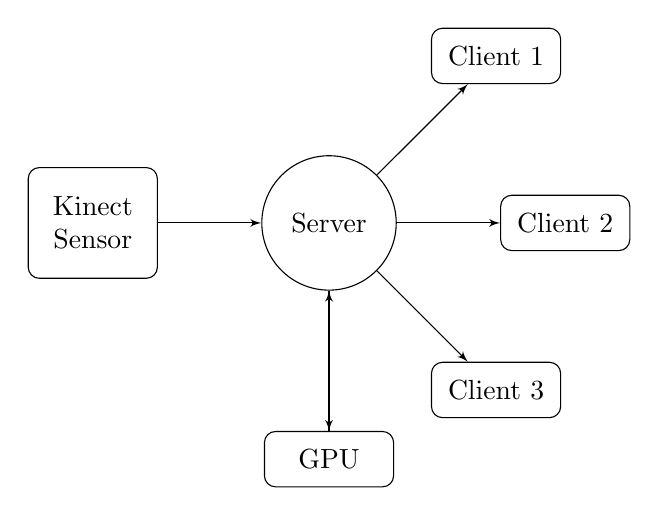
\begin{tikzpicture}[node distance = 3cm, auto]
        \node [bigbox] (kinect) {Kinect Sensor};
        \node [round, right of=kinect] (server) {Server};
        \node [smallbox, below of=server] (gpu) {GPU};
        \node [smallbox, right of=server] (client2) {Client 2};
        \node [smallbox, above right of=server] (client1) {Client 1};
        \node [smallbox, below right of=server] (client3) {Client 3};

        \path [line] (kinect) -- (server);
        \path [line] (server) -- (gpu);
        \path [line] (gpu) -- (server);
        \path [line] (server) -- (client1);
        \path [line] (server) -- (client2);
        \path [line] (server) -- (client3);
      \end{tikzpicture}
      \caption{Software infrastructure event flowchart depicting the Kinect sensor interfacing with three clients via the server.\label{fig:pipeline}}
    \end{figure}
    The software is conceptualized as a hybrid client capable of supporting multiple connections. The back-end is written in a low-level language that interfaces directly with the Kinect (via the Microsoft Kinect API) and uses the workstation's graphical processing unit (GPU) to convert raw sensor data into well-formed intermediate output. The intention is to offload processor-intensive computations to the workstation and stream the output to the front-end, which is a modular, lightweight application with little to no dependencies. The front-end consumes the output and renders graphical content to the user's display. Figure~\ref{fig:pipeline} depicts the flow of data from the Kinect sensor to the server, where it is interpreted before being piped to connected user clients.

    Establishing the software as a dichotomy of a front-end and back-end allows for the front-end to be adapted for different applications, treating the output from the server as a black-boxed ``bag-of-features''. In addition, since the Microsoft Kinect API is still under development, new changes can be slipstreamed into the back-end without further modification to the rest of the software infrastructure.
  \section{Road-map}
    \renewcommand{\thesubsection}{\Roman{subsection}}
    Due to the projected scale of this project, the erratic nature of the academic semester, and the ongoing development of the Kinect sensor, we define project milestones as a series of phases to be attempted in due course, or postponed (as may be required) until the underlying technology is sufficiently mature.
    \subsection{Core Functionality\label{sec:phase1}}
      The Kinect API tracks 21 3-D joint coordinates of the human skeleton model in real-time (30 frames/sec), corresponding to the spatial location of a user in the Kinect sensor's FOV. This polling rate generates $21 \times 30 \times 3 = 1890$ real-valued skeleton model coordinates per second. In addition, the skeleton model is robust to variation in the shape and size of the human body, color and texture of clothing, and objects or surfaces in the background, thus we omit consideration for these variables (otherwise considered anomalies) in the design of our action model representation.

      \begin{figure}[ht!]
        \centering
        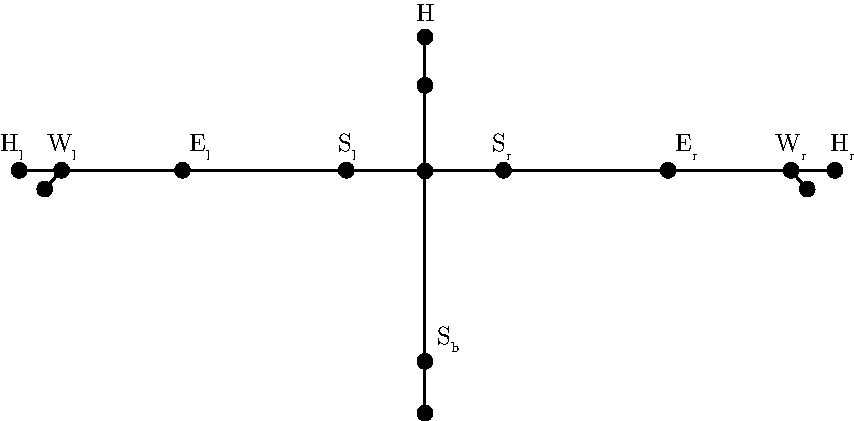
\includegraphics[width=0.75\textwidth]{img/Body}
        \caption{Partial joint nomenclature for the Kinect Skeleton Model, showing the top half of the body. Joints of interest are labeled, where $H$ corresponds to the head, $S_{\{ l,r \}}$ corresponds to the left or right shoulder, $E_{\{ l,r \}}$ corresponds to the left or right elbow, $W_{\{ l,r \}}$ corresponds to the left or right wrist, $H_{\{ l,r \}}$ corresponds to the left or right hand, and $S_b$ corresponds to the base of the spine.\label{fig:jointnomenclature}}
      \end{figure}
      Since our implementation is gesture-based, the skeleton model can be simplified to focus only on coordinates above the base of the spine. The most pertinent joints are the left and right hand, left and right wrist, left and right elbow, and left and right shoulder. Figure~\ref{fig:jointnomenclature} assigns labels to these joints for ease of reference in subsequent discussions.
    \subsection{Establishing Coherence\label{sec:phase2}}
      In this phase, we establish the backbone of the connection between the Kinect and the front-end client.
      \subsubsection{Fleck WebSockets Server}
      The Kinect API runs on an open-source C\# WebSockets server branched from the Nugget project\footnote{\url{https://github.com/statianzo/Fleck}}. The server processes frame data from the Kinect and compiles joint coordinate information into a JSON packet, which is compressed and sent to all connected clients. Due to the nature of the Kinect API, the server encapsulates and runs the KinectService executable (\verb|KinectService.exe|) as a core dependency for interfacing with the Kinect at the USB hardware level.
      \subsubsection{HTML5 WebSockets API}
      The front-end client interfaces with the C\# WebSockets server using the inbuilt HTML5 WebSockets API\footnote{\url{http://www.w3.org/TR/2011/WD-websockets-20110419/}}. An exponential back-off algorithm was also utilized to multiplicatively decrease the rate of connection attempts in the event that a connection fails. The front-end opens a TCP connection to the C\# server, accepting and parsing JSON packets via a duplex channel for direct consumption by the client interface. The front-end only listens passively, and does not establish a heartbeat connection with the back-end since there is no synchronization needed.
      \subsubsection{Viewport Nomenclature}
      Subsequent discussions necessarily reference multiple coordinate systems. The Kinect's TOF laser returns depth measurements in units of millimeters, which are converted to pixel values in the frame of reference of the Kinect's FOV. Since the dimensions of the Kinect's FOV differ from the dimensions of the screen on which the application is being utilized, a mapping must be defined from one coordinate system to the other. To disambiguate, the coordinate space in the Kinect's FOV is referred to as the ``Kinect viewport'', $V_k$, and the coordinate space of the screen as the ``screen viewport'', $V_s$. We also define in the next section a ``user viewport'', $V_u$, which scopes the user's gestures to a subset of the Kinect viewport.
    \subsection{Gestural Interaction\label{sec:phase3}}
      As a simple nomenclature which we will build upon in this section, we classify gestures as either \emph{arm-level} gestures or \emph{hand-level} gestures. Eponymously, arm-level gestures involve the movement of the entire arm, such as pushing, pulling, or swiping actions. Hand-level gestures involve the movement of only the hand, such as expanding all fingers to show an open palm, clenching all fingers to form a fist, or extending a single finger to point in a direction.

      Interaction with the system begins when the sensor detects a predefined static pose. This enables the algorithm's initial detection algorithm to be memoryless, i.e.~only the current frame needs to be analyzed. Once the pose has been detected, the algorithm begins tracking and caching the location of the hand joints in order to facilitate cursor manipulation feedback on-screen. Listeners on the cache detect when a series of frames fulfill the constraints required to construe them as a gesture, and call the appropriate subroutines at the application level.
      \subsection{Trigger Mechanism}
      In practice, gesture recognition must be applied to a finite data-set (e.g.~a video segment), in which the algorithm returns all statistically significant occurrences of a gesture within the data-set. In such cases, it is trivial to repeatedly expand a window of analysis to include frames before and after a suspected gesture component. However, it is not possible to deterministically identify a gesture when incoming data arrives as a stream, because the subsequent frames of data are unknown to the algorithm. We overcome this difficulty by constraining the initial set of permissible actions to the raising of the left or right hand above shoulder height. Specifically we define the constraints:
      \begin{align}
        x_{S_r} &\leq x_{W_r} \leq x_{E_r} \\
        y_{S_r} &\geq y_{W_r} \geq y_{E_r}
      \end{align}
      for detecting a raised right hand, and similarly:
      \begin{align}
        x_{S_l} \leq x_{W_l} \leq x_{E_l} \\
        y_{S_l} \geq y_{W_l} \geq y_{E_l}
      \end{align}
      for detecting a raised left hand. The fulfillment of either set of constraints constitutes a start gesture. When a start gesture is detected, control for the gesture recognition algorithm is handed to the cursor manipulation subroutine. The intuition for this gesture is that it is unlikely for a user to raise a hand above shoulder height in normal conversation while facing the sensor, thus preventing cursor manipulation from happening accidentally

      A constraint that codifies a gesture for stopping the cursor manipulation subroutine can also be defined. While it is possible to continue receiving input indefinitely, we account for a situation in which it may be advantageous to neglect any bodies in front of the sensor (until the start gesture is detected once again). The constraints are defined as follows:
      \begin{align}
        y_{H_l} \geq y_{S_b} \label{eq:stop1} \\
        y_{H_r} \geq y_{S_b} \label{eq:stop2}
      \end{align}
      The fulfillment of both constraints constitutes a stop gesture. When a stop gesture is detected, control for the gesture recognition algorithm is handed back to the start gesture detection subroutine. The intuition for this gesture is that dropping both hands below the waist is a natural action that represents a lack of further intention to interact with the software.
      \subsubsection{Cursor Manipulation}
      The ``cursor'' on-screen is represented by a pair of circles corresponding to the position of the user's hands within a region --- the user viewport --- defined as a subset of the Kinect viewport. A subset, rather than the entirety of the Kinect viewport, is utilized firstly because the wide-angle FOV of the Kinect sensor is capable of acquiring a region that is larger than the arm-span of the user, and secondly with the view of maintaining good ergonomics in the course of user interaction. A direct mapping of the Kinect viewport to the screen viewport would require the user to walk across some or all of the FOV of the sensor (depending on the user's proximity to the sensor) in order to move the cursor from one edge of the screen viewport to the other. In contrast, localizing the mapping using the user viewport, instead of the Kinect viewport, allows the user's hands to span the screen viewport without fully extending the arm.

      \begin{figure}[ht!]
        \centering
        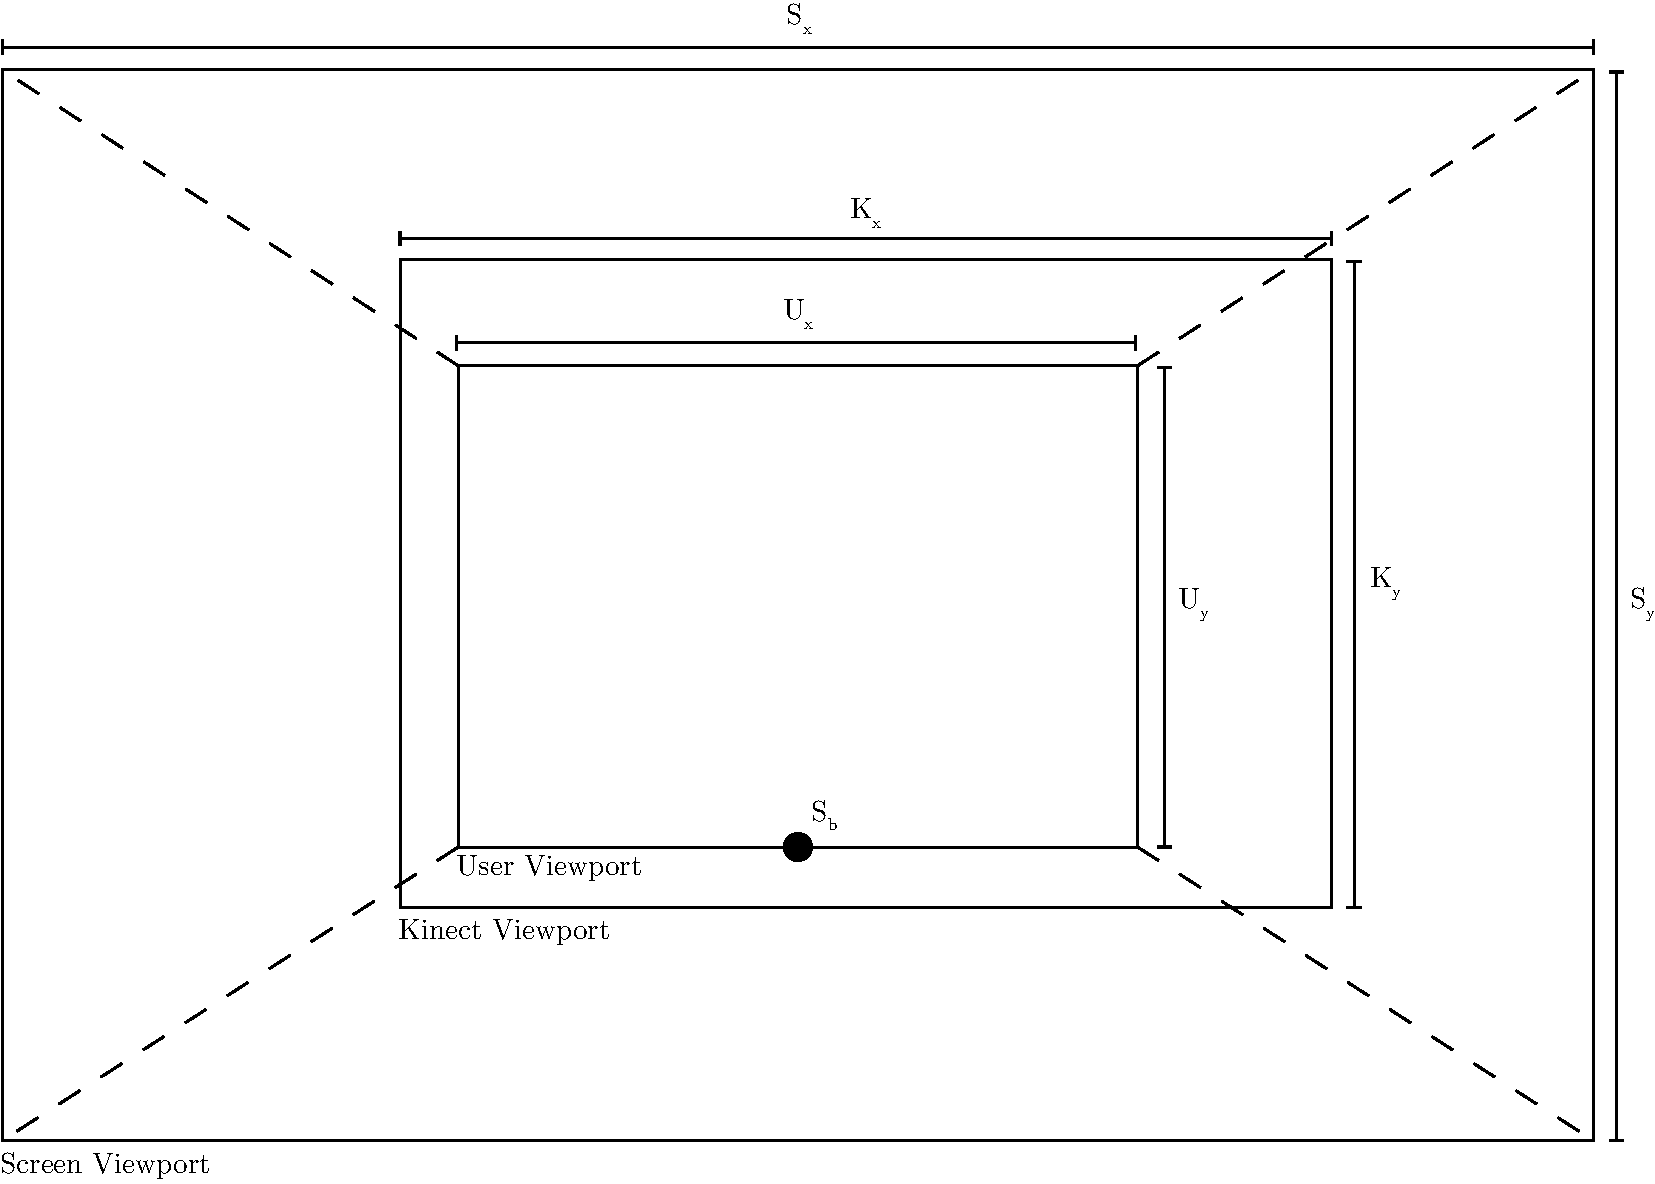
\includegraphics[width=0.8\textwidth]{img/Mapping}
        \caption{An overview of the different viewports and their respective dimensions. $V_u$, with dimensions $U_x$ and $U_y$, is a subset of $V_k$, with dimensions $K_x$ and $K_y$. Every point in $V_u$ maps to a corresponding point in $V_s$, with dimensions $S_x$ and $S_y$.\label{fig:mapping}}
      \end{figure}
      Fig.~\ref{fig:mapping} describes the relationship between the different viewports. The Kinect viewport $V_k$ has fixed dimensions $K_x = 512\textrm{px}$ and $K_y = 424\textrm{px}$, which are hardware specifications. Within $V_k$, we define $V_u \in V_k$ such that $V_u$ has dimensions $U_x$ and $U_y$. $U_x$ is calculated from the adjusted arm-span of the user:
      \begin{equation}
        U_x = \left|\frac{1}{2}(x_{E_l}-x_{W_l}) + (x_{S_l} - x_{E_l})\right| + \left|\frac{1}{2}(x_{E_r}-x_{W_r}) + (x_{S_r} - x_{E_r})\right| + \left| x_{S_l} - x_{S_r} \right|
      \end{equation}
      where we are summing the inter-shoulder distance and the distance from each shoulder to the middle of the forearm. The rationale for using the middle of the forearm instead of considering the fully extended arm-span is that requiring the user to fully extend his or her arm in order to reach the edge of the screen will result in significant discomfort over prolonged usage. Similarly, the height $U_y$ is calculated by measuring the height of the user, in the form of the distance from the user's spine base to the top of the head:
      \begin{equation}
        U_y = \left|(y_H - y_{S_b}) + (y_H - y_N)\right|
      \end{equation}
      where we utilize the distance from the head to the neck to account for the distance from the head coordinate (which is in fact the center of the head) to the top of the head. The base of the user viewport is centered at the user's spine base. This localizes the system such that cursor manipulation is affected only by the location of the user's hands relative to their spine base, and not to their absolute position in the Kinect viewport. Fig~\ref{fig:userviewport} provides a graphical depiction of the user viewport overlaid on a simplified skeleton model showing only pertinent joints.
      \begin{figure}[ht!]
        \centering
        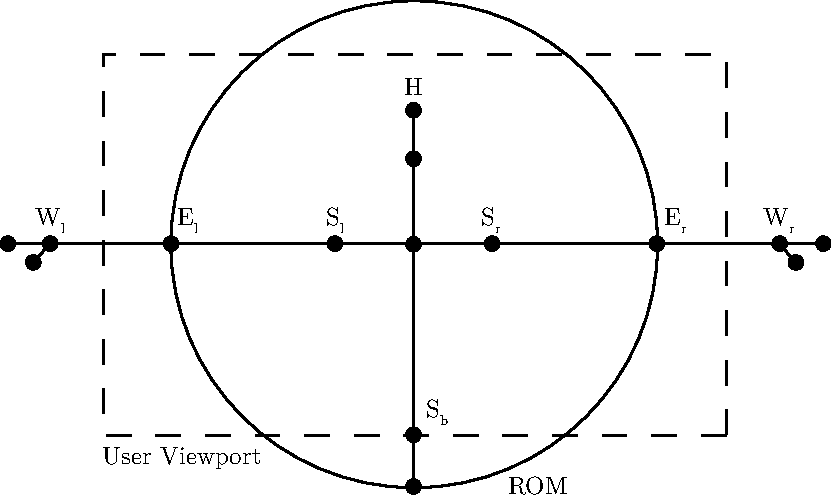
\includegraphics[width=0.8\textwidth]{img/User-Viewport}
        \caption{The position of a skeleton relative to the user viewport, $V_u$ as defined.\label{fig:userviewport}}
      \end{figure}
      \begin{figure}[ht!]
        \centering
        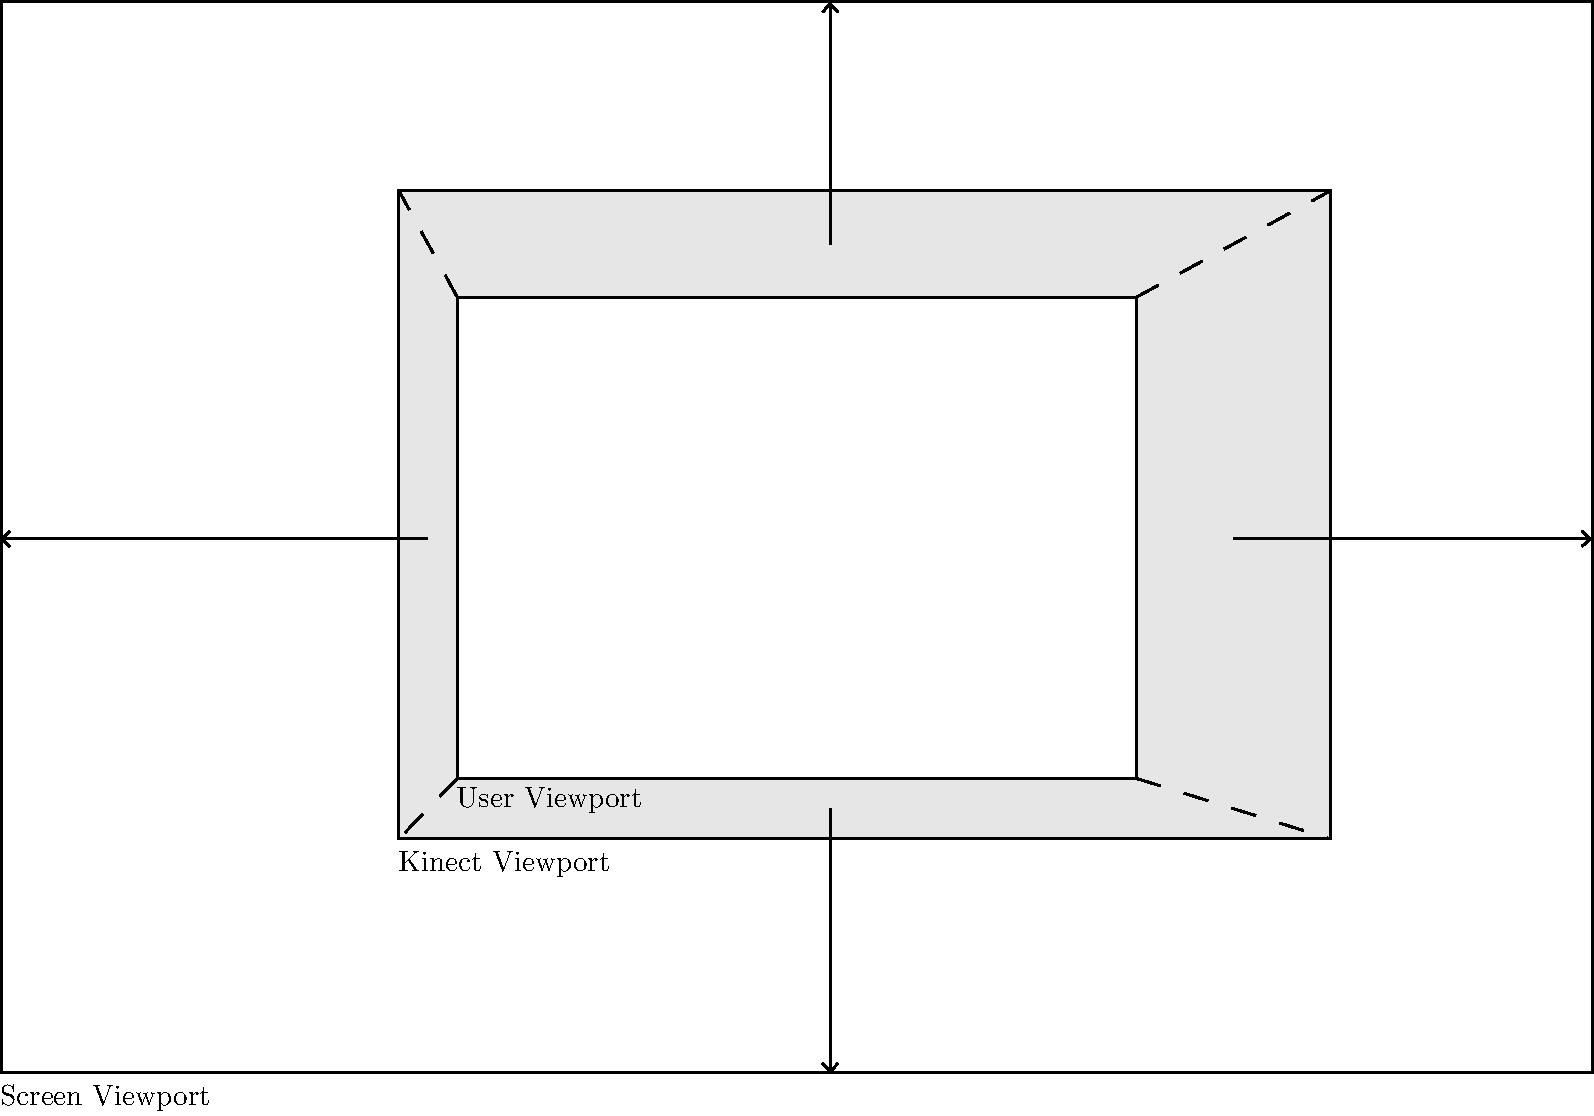
\includegraphics[width=0.8\textwidth]{img/Clipping}
        \caption{Coordinate clipping when the user's hand extends outside the user viewport $V_u$ but is still detected because it is within the Kinect's viewport $V_k$. Coordinates in the gray region are clipped to the edge of the screen.\label{fig:clipping}}
      \end{figure}

      The mapping from the user viewport to the screen viewport is performed using a piecewise function, to account for the case in which the user's hands extend outside the user's viewport, but remain within the Kinect viewport (and hence are still detected). As follows, for some coordinate $(x_{V_u},y_{V_u}) \in V_u$ representing the location of a tracked hand, the corresponding coordinates $(x_{V_s},y_{V_s}) \in V_s$ are:
      \begin{align*}
        x_{V_s} &=
        \begin{cases}
          \dfrac{x}{U_x}S_x, &\quad 0 \leq x \leq U_x \\
          0, &\quad x < 0 \\
          S_x, &\quad x > U_x
        \end{cases} \\
        y_{V_s} &=
        \begin{cases}
          \dfrac{y}{U_y}S_y, &\quad 0 \leq y \leq U_y \\
          0, &\quad y < 0 \\
          S_y, &\quad y > U_y
        \end{cases}
      \end{align*}
      where $S_x$ and $S_y$ are dimensions of the user's screen acquired at run time. Fig.~\ref{fig:clipping} provides a graphical depiction of how clipping is handled.
      \subsubsection{Hand States}
      Native support for hand state detection is provided by the Kinect API. The default ``open'' state corresponds to an unobstructed palm with all fingers extended. This state is used solely for cursor movement on-screen. The ``closed'' state corresponds to a grabbing action made by clenching all fingers to form a fist. This state is used to validate a pull or push gesture, synonymous with pulling or pushing an object in reality. The interface provides feedback that a closed gesture is detected by decreasing the size of the cursor circle. The ``point'' state corresponds either to only the extended index finger, or both the extended index and middle finger held apart. This interface provides feedback that a point gesture is detected by decreasing the size of the cursor circle to a tiny point, and increases the sensitivity of the cursor circle on-screen. The effect of the point gesture is to produce a point suitable for annotation or identification of fine details.
      \subsubsection{Pulling and Pushing}
      Pulling and pushing are gestures defined by a respective increase or decrease in the z-component of a closed hand coordinate. The exact behavior of the pull and push gesture at the interface level is left to the discretion of the user.
      % \subsubsection{Swiping}
      % \subsubsection{Jitter and Tremor}
    % \subsection{Content Development\label{sec:phase4}}
      % \emph{This section provides a speculative overview of work that may be conducted this area, and will be updated as more information becomes available.}
    \subsection{Testing and Robustness Evaluation\label{sec:phase5}}
      \emph{This section provides a speculative overview of work that may be conducted this area, and will be updated as more information becomes available.}

      Code base development up till this point has focused on the authoring of specifications that enable the creation of a prototype and proof of concept. As the project proceeds and the code base expands, it is imperative that a battery of tests (at both the unit level and regression level) are introduced to account for the wide range of circumstances which the software may encounter. Front-end testing can be expediently implemented using QUnit, and back-end testing can be implemented, in part, by using the Kinect Fusion library to record and replay frame data.
    \subsection{User Recognition\label{sec:phase6}}
      \emph{This section provides a speculative overview of work that may be conducted this area, and will be updated as more information becomes available.}

      The Kinect API is capable of performing biometric recognition using data from the IR sensor. While this feature has not been implemented in the API at time of writing, it presents significant advantages for handling saliency and user control in an environment where the Kinect may detect and track multiple skeletons. For example, the Kinect should only acquire input from a lecturer in a crowded classroom, and ignore any students who may have hands raised.

      An alternative solution is to exploit the audio beam-forming capability of the Kinect's microphone array. This would serve as a passive method of identifying the user in control of the system, by acquiring input which is closest to the audio source determined by beam-forming.
  \section{Deliverables}
      Literature review and familiarization with the hardware will be completed by 27th January. Phase~\ref{sec:phase1} is expected to be completed by the 24th of February, presented as a standalone application (or cannibalized example) capturing and returning joint coordinate data. Phase~\ref{sec:phase2} is expected to be completed by the 31st of March, presented as a simple interface between a scaffolding front-end application and a bare-bones server implementation. Phase~\ref{sec:phase3} and content development are expected to be completed by the 28th of April, presented as a package capable of detecting user gestures and providing feedback for these gestures in the form of interactivity on the front-end application. Phase~\ref{sec:phase5} is expected to be completed by the end of the semester, presented as as full code-base documentation accompanied by unit and regression tests. Any remaining time thereafter will be dedicated to preliminary work in Phase~\ref{sec:phase6}
  \section{Acknowledgments}
    The authors are indebted to Donald Greenberg, Joe Kider, John Decorato, and Jeremy Newlin for advice and assistance rendered throughout the course of the project. This work was supported by the Cornell Program of Computer Graphics.
\end{document}
